\paragraph{} 

\begin{figure}[]
    \centering
    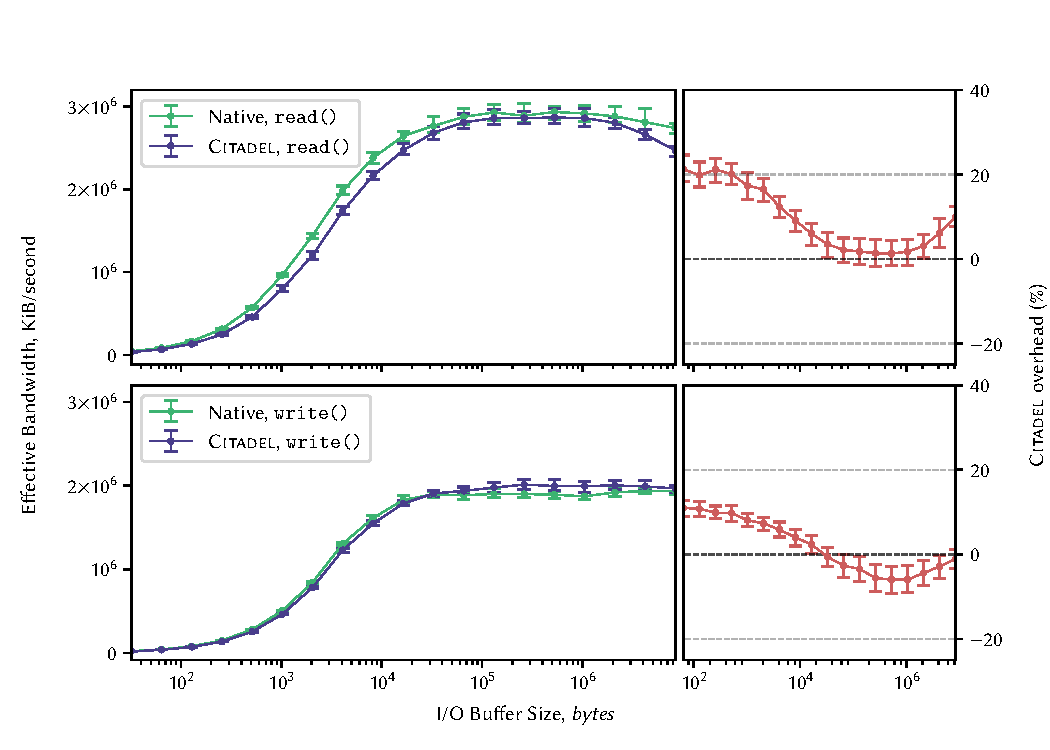
\includegraphics[width=\linewidth]{figures/graphs/io.pdf}
    \vspace{-5mm}
    \caption[Effective \texttt{read()/write()} bandwidths for both the native Linux kernel and \textsc{Citadel}.]{Effective \texttt{read()/write()} bandwidths for both the native Linux kernel and \textsc{Citadel}. The Percentage overhead is also presented.}
    \label{fig:io-graph}
\end{figure}


\begin{figure}[]
    \centering
    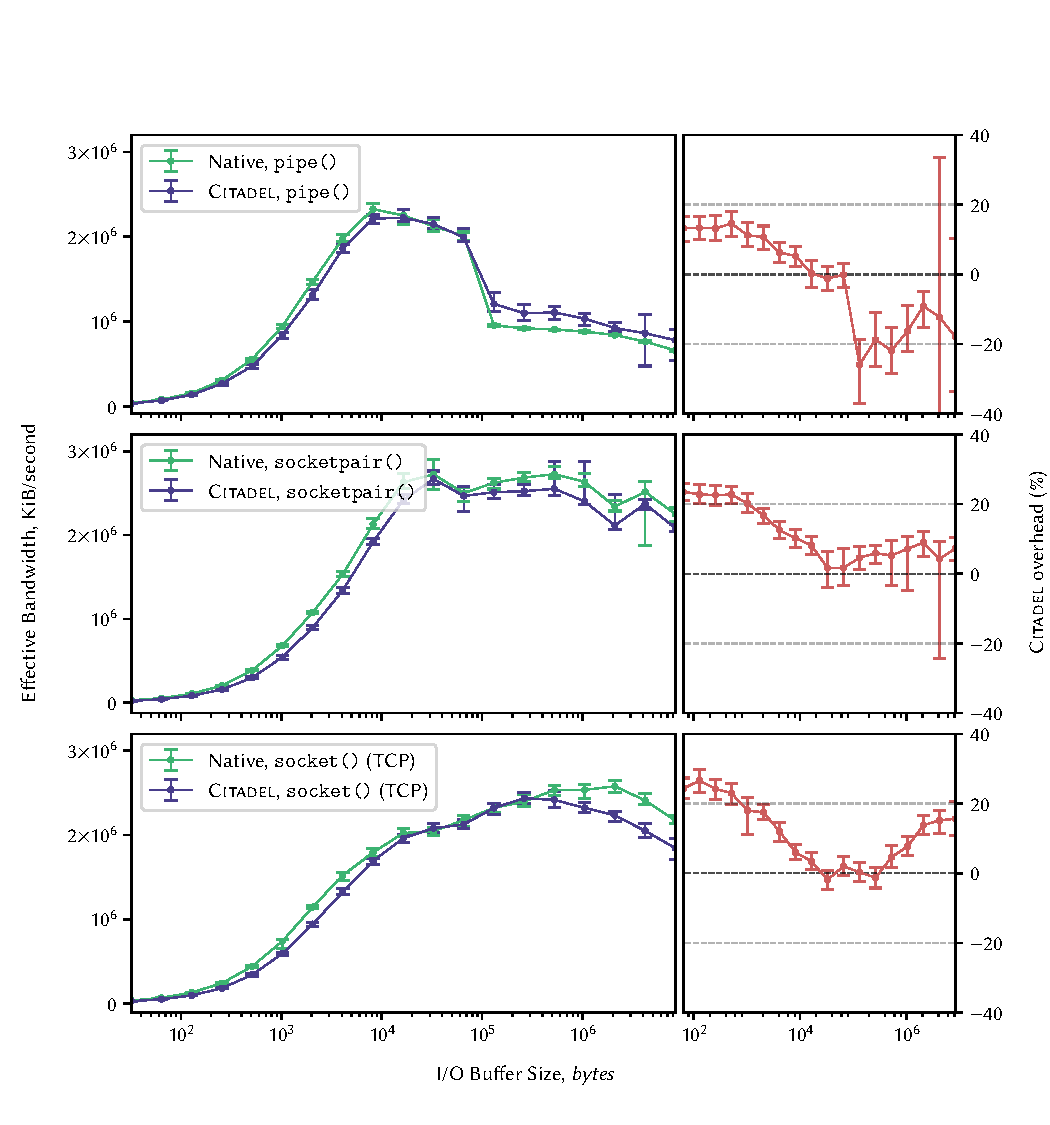
\includegraphics[width=\linewidth]{figures/graphs/ipc-2thread.pdf}
    \vspace{-5mm}
    \caption{Effective bandwidths for various types of IPC between \textit{2 threads}.}
    \label{fig:ipc-2thread-graph}
\end{figure}


\begin{figure}[]
    \centering
    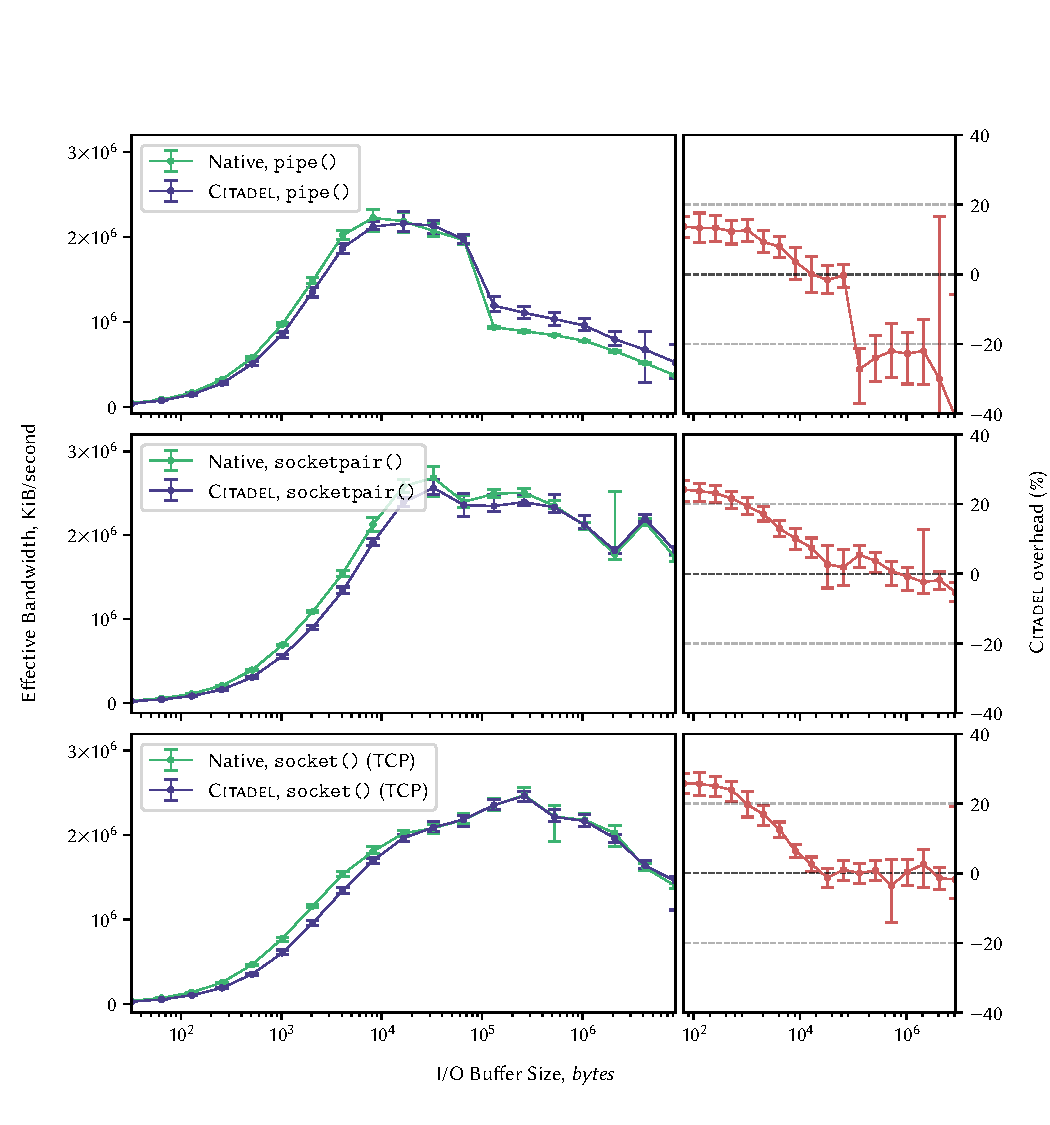
\includegraphics[width=\linewidth]{figures/graphs/ipc-2proc.pdf}
    \vspace{-5mm}
    \caption{Effective bandwidths for various types of IPC between \textit{2 processes}.}
    \label{fig:ipc-2proc-graph}
\end{figure}